%
% Template Laporan Skripsi/Thesis 
%
% @author  Andreas Febrian, Lia Sadita 
% @version 1.03
%
% Dokumen ini dibuat berdasarkan standar IEEE dalam membuat class untuk 
% LaTeX dan konfigurasi LaTeX yang digunakan Fahrurrozi Rahman ketika 
% membuat laporan skripsi. Konfigurasi yang lama telah disesuaikan dengan 
% aturan penulisan thesis yang dikeluarkan UI pada tahun 2008.
%

%
% Tipe dokumen adalah report dengan satu kolom. 
%
\documentclass[12pt, a4paper, onecolumn, oneside, final]{report}

% Load konfigurasi LaTeX untuk tipe laporan thesis
\usepackage{_internals/uithesis}

% Daftar pemenggalan suku kata dan istilah dalam LaTeX
%
% Hyphenation untuk Indonesia 
%
% @author  Andreas Febrian
% @version 1.00
% 
% Tambahkan cara pemenggalan kata-kata yang salah dipenggal secara otomatis 
% oleh LaTeX. Jika kata tersebut dapat dipenggal dengan benar, maka tidak 
% perlu ditambahkan dalam berkas ini. Tanda pemenggalan kata menggunakan 
% tanda '-'; contoh:
% menarik
%   --> pemenggalan: me-na-rik
%

\hyphenation{
    % alphabhet A
    a-na-li-sa a-tur 
    a-pli-ka-si 
    % alphabhet B
    ba-ngun-an 
    be-be-ra-pa 
    ber-ge-rak
    ber-ke-lan-jut-an 
    ber-pe-nga-ruh 
    % alphabhet C
    ca-ri
    % alphabhet D
    di-sim-pan di-pim-pin de-ngan da-e-rah di-ba-ngun da-pat di-nya-ta-kan 
    di-sim-bol-kan di-pi-lih di-li-hat de-fi-ni-si
    % alphabhet E
    e-ner-gi eks-klu-sif
    % alphabhet F
    fa-si-li-tas
    % alphabhet G
    ga-bung-an ge-rak
    % alphabhet H
    ha-lang-an
    % alphabhet I
    % alphabhet J
    % alphabhet K
    ke-hi-lang-an
    ku-ning 
    kua-li-tas ka-me-ra ke-mung-kin-an ke-se-pa-ham-an
    % alphabhet L
    ling-kung-an
    % alphabhet M
    me-neng-ah
    meng-a-tas-i me-mung-kin-kan me-nge-na-i me-ngi-rim-kan 
    meng-u-bah meng-a-dap-ta-si me-nya-ta-kan mo-di-fi-ka-si
    meng-a-tur
    % alphabhet N
    nya-ta non-eks-klu-sif
    % alphabhet O
    % alphabhet P
	pe-nye-rap-an 
	pe-ngon-trol
    pe-mo-del-an
    pe-ran  pe-ran-an-nya
    pem-ba-ngun-an pre-si-den pe-me-rin-tah prio-ri-tas peng-am-bil-an 
    peng-ga-bung-an pe-nga-was-an pe-ngem-bang-an 
    pe-nga-ruh pa-ra-lel-is-me per-hi-tung-an per-ma-sa-lah-an 
    pen-ca-ri-an peng-struk-tur-an
    % alphabhet Q
    % alphabhet R
    ran-cang-an
    % alphabhet S
    si-mu-la-si sa-ngat
    % alphabhet T
    te-ngah
    ter-da-pat
    % alphabhet U
    % alphabhet V
    % alphabhet W
    % alphabhet X
    % alphabhet Y
    % alphabhet Z
    % special
}

% Load konfigurasi khusus untuk laporan yang sedang dibuat
%-----------------------------------------------------------------------------%
% Informasi Mengenai Dokumen
%-----------------------------------------------------------------------------%
% 
% Judul laporan. 
\var{\judul}{Network Automation}
% 
% Tulis kembali judul laporan, kali ini akan diubah menjadi huruf kapital
\Var{\Judul}{NETWORK AUTOMATION}
% 
% Tulis kembali judul laporan namun dengan bahasa Ingris
\var{\judulInggris}{Network Automation}

% 
% Tipe laporan, dapat berisi Skripsi, Tugas Akhir, Thesis, atau Disertasi
\var{\type}{Tugas AKPSI}
% 
% Tulis kembali tipe laporan, kali ini akan diubah menjadi huruf kapital
\Var{\Type}{Tugas AKPSI}
% 
% Tulis nama penulis 
\var{\penulis}{Nama Penulis}
% 
% Tulis kembali nama penulis, kali ini akan diubah menjadi huruf kapital
\Var{\Penulis}{Nama Penulis}
% 
% Tulis NPM penulis
\var{\npm}{NPM}
% 
% Tuliskan Fakultas dimana penulis berada
\Var{\Fakultas}{Ilmu Komputer}
\var{\fakultas}{Ilmu Komputer}
% 
% Tuliskan Program Studi yang diambil penulis
\Var{\Program}{MAGISTER TEKNOLOGI INFORMASI}
\var{\program}{Magister Teknologi Informasi}
% 
% Tuliskan tahun publikasi laporan
\Var{\bulan}{Desember}
\Var{\tahun}{2024}
% 
% Tuliskan gelar yang akan diperoleh dengan menyerahkan laporan ini
\var{\gelar}{Magister Teknologi Informasi}
% 
% Tuliskan tanggal pengesahan laporan, waktu dimana laporan diserahkan ke 
% penguji/sekretariat
\var{\tanggalPengesahan}{XX Juli 2019} 
% 
% Tuliskan tanggal keputusan sidang dikeluarkan dan penulis dinyatakan 
% lulus/tidak lulus
\var{\tanggalLulus}{XX Juli 2019}
% 
% Tuliskan pembimbing 
\var{\pembimbing}{Prof. ???}
% 
% Alias untuk memudahkan alur penulisan paa saat menulis laporan
\var{\saya}{Penulis}

%-----------------------------------------------------------------------------%
% Judul Setiap Bab
%-----------------------------------------------------------------------------%
% 
% Berikut ada judul-judul setiap bab. 
% Silahkan diubah sesuai dengan kebutuhan. 
% 
\Var{\kataPengantar}{Kata Pengantar}
\Var{\babSatu}{BUSINESS REQUIREMENT}
\Var{\babDua}{FEASIBILITY ANALISIS}
\Var{\babTiga}{PROJECT PLAN}
\Var{\babEmpat}{REQUIREMENTS DEFINITION}
\Var{\babLima}{REQUIREMENT ANALYSIS STRATEGY}
\Var{\babEnam}{FUNCTIONAL MODELS}
\Var{\babTujuh}{STRUCTURAL MODELS}
\Var{\babDelapan}{BEHAVIORAL MODELS}
\Var{\babSembilan}{USER INTERFACE LAYER DESIGN}
\Var{\babSepuluh}{PHYSICAL ARCHITECTURE LAYER DESIGN}
\Var{\babSebelas}{WORKING SYSTEM PROTOTYPE}
\Var{\babDuabelas}{TESTING}
\Var{\babTigabelas}{INSTALLATION AND OPERATIONS}

\Var{\kesimpulan}{Kesimpulan dan Saran}

% Daftar istilah yang mungkin perlu ditandai 
%
% @author  Andreas Febrian
% @version 1.00
% 
% Mendaftar seluruh istilah yang mungkin akan perlu dijadikan 
% italic atau bold pada setiap kemunculannya dalam dokumen. 
% 

\var{\license}{\f{Creative Common License 1.0 Generic}}
\var{\bslash}{$\setminus$}

% Awal bagian penulisan laporan
\begin{document}
%
% Sampul Laporan
% %
% Sampul Laporan

%
% @author  unknown
% @version 1.01
% @edit by Andreas Febrian
%

\begin{titlepage}
    \begin{center}    
        \begin{figure}
            \begin{center}
                
\includegraphics[width=2.5cm]{_internals/makara.eps}
            \end{center}
        \end{figure}    
        \vspace*{0cm}
        \bo{
        	UNIVERSITAS INDONESIA\\
        }
        
        \vspace*{1.0cm}
        % judul thesis harus dalam 14pt Times New Roman
        \bo{\Judul} \\[1.0cm]

        \vspace*{2.5 cm}    
        % harus dalam 14pt Times New Roman
        \bo{\Type}

        \vspace*{3 cm}       
        % penulis dan npm
        \bo{\Penulis} \\
        \bo{\npm} \\

        \vspace*{5.0cm}

        % informasi mengenai fakultas dan program studi
        \bo{
        	FAKULTAS \Fakultas\\
        	PROGRAM STUDI \Program \\
        	DEPOK \\
        	\tahun
        }
    \end{center}
\end{titlepage}


%
% Gunakan penomeran romawi
\pagenumbering{roman}

%
% load halaman judul dalam
\addChapter{HALAMAN JUDUL}
%
% Halaman Judul Laporan 
%
% @author  unknown
% @version 1.01
% @edit by Andreas Febrian
%

\begin{titlepage}
    \begin{center}\begin{figure}
            \begin{center}
                
\includegraphics[width=2.5cm]{_internals/makara.eps}
            \end{center}
        \end{figure}    
        \vspace*{0cm}
        \bo{
        	UNIVERSITAS INDONESIA\\
        }
        
        \vspace*{1.0cm}
        % judul thesis harus dalam 14pt Times New Roman
        \bo{\Judul} \\[1.0cm]

        \vspace*{2.5 cm}    
        % harus dalam 14pt Times New Roman
        \bo{\Type} \\
        % keterangan prasyarat
        % \bo{Diajukan sebagai salah satu syarat untuk memperoleh gelar \\
        % \gelar}\\

        \vspace*{3 cm}       
        % penulis dan npm
        % \bo{\Penulis} \\
        % \bo{\npm} \\
        
        \bo{Muh Hatta Eka Putra	- 2406386425}\\
        \bo{Jon Felix Germinian	- 2406473192}\\
        \bo{Muhammad Irfan J	- 2406473305}\\
        \bo{Namirah Alisya		- 2406473324}\\
        \bo{Tio Ramadhan		- 2406473450}\\
        


        \vspace*{5.0cm}

        % informasi mengenai fakultas dan program studi
        \bo{
        	FAKULTAS \Fakultas\\
        	PROGRAM STUDI \Program \\
        	SALEMBA \\
        	\bulan\ \tahun
        }
    \end{center}
\end{titlepage}

%
% setelah bagian ini, halaman dihitung sebagai halaman ke 2
\setcounter{page}{2}

%
% load halaman pengesahan
% \addChapter{LEMBAR PERSETUJUAN}
% %
% Halaman Pengesahan
%
% @author  Andreas Febrian
% @version 1.01
%

\chapter*{HALAMAN PERSETUJUAN}

\vspace*{0.2cm}
\noindent 

\noindent
\begin{tabular}{l l p{11cm}}
	\bo{Judul}&: & \judul \\ 
	\bo{Nama}&: & \penulis \\
	\bo{NPM}&: & \npm \\
\end{tabular} \\

\vspace*{1.2cm}

\noindent Laporan \type~ini telah diperiksa dan disetujui.\\[0.3cm]
\begin{center}
\tanggalPengesahan \\[2cm]


\underline{\pembimbing}\\[0.1cm]
Pembimbing \type
\end{center}

\newpage
%
% load halaman orisinalitas 
% \addChapter{LEMBAR PERNYATAAN ORISINALITAS}
% %
% Halaman Orisinalitas
%
% @author  Andreas Febrian
% @version 1.01
%

\chapter*{Halaman Pernyataan Orisinalitas}
\vspace*{2cm}

\begin{center}
	\bo{\type~ini adalah hasil karya saya sendiri, \\ 
	dan semua sumber baik yang dikutip maupun dirujuk \\
	telah saya nyatakan dengan benar.} \\
	\vspace*{2.6cm}
	
	\begin{tabular}{l c l}
	\bo{Nama} & : & \bo{\penulis} \\
	\bo{NPM} & : & \bo{\npm} \\ 
	\bo{Tanda Tangan} & : & \\
	& & \\
	& & \\
	\bo{Tanggal} & : & \bo{\tanggalPengesahan} \\	
	\end{tabular}
\end{center}

\newpage
%
%
% \addChapter{LEMBAR PENGESAHAN}
% %
% Halaman Pengesahan Sidang
%
% @author  Andreas Febrian, Andre Tampubolon 
% @version 1.02
%

\chapter*{HALAMAN PENGESAHAN}

\vspace*{0.4cm}
\noindent 

\noindent
\begin{tabular}{ll p{9cm}}
	\type~ini diajukan oleh&: & \\
	Nama&: & \penulis \\
	NPM&: & \npm \\
	Program Studi&: & \program \\
	Judul \type&: & \judul \\
\end{tabular} \\

\vspace*{1.0cm}

\noindent \bo{Telah berhasil dipertahankan di hadapan Dewan Penguji 
dan diterima sebagai bagian persyaratan yang diperlukan untuk 
memperoleh gelar \gelar~pada Program Studi \program, Fakultas 
\fakultas, Universitas Indonesia.}\\[0.2cm]

\begin{center}
	\bo{DEWAN PENGUJI}
\end{center}

\vspace*{0.3cm}

\begin{tabular}{l l l l }
	& & & \\
	Pembimbing&: & \pembimbing & (\hspace*{3.0cm}) \\
	& & & \\
	Penguji&: & Prof. XXX & (\hspace*{3.0cm}) \\
	& & & \\
	Penguji&: & Prof. XXXX & (\hspace*{3.0cm}) \\
	& & & \\
	Penguji&: & Prof. XXXXXX & (\hspace*{3.0cm}) \\
\end{tabular}\\

\todo{Jangan lupa mengisi nama para penguji.}

\vspace*{2.0cm}

\begin{tabular}{ll l}
	Ditetapkan di&: & Depok\\
	Tanggal&: & \tanggalLulus \\
\end{tabular}


\newpage
%
%
% \addChapter{\kataPengantar}
% %-----------------------------------------------------------------------------%
\chapter*{Kata Pengantar}
%-----------------------------------------------------------------------------%
Template ini disediakan untuk orang-orang yang berencana menggunakan 
\latex~untuk membuat dokumen tugas akhirnya. 
Mengapa \latex? 
Ada banyak hal mengapa menggunakan \latex, diantaranya:

\begin{enumerate}
	\item \latex~membuat kita jadi lebih fokus terhadap isi dokumen, bukan 
		tampilan atau halaman. 
	\item \latex~memudahkan dalam penulisan persamaan matematis. 
	\item Adanya automatis dalam penomoran caption, bab, subbab, subsubbab, 
		referensi, dan rumus. 
	\item Adanya automatisasi dalam pembuatan daftar isi, daftar gambar, dan
		daftar tabel. 
	\item Adanya kemudahan dalam memberikan referensi dalam tulisan dengan 
		menggunakan label. Cara ini dapat meminimalkan kesalahan pemberian 
		referensi. 
\end{enumerate}

Template ini bebas digunakan dan 
didistribusikan sesuai dengan aturan \license, yang secara sederhana berisi: 

\begin{figure}
	\centering
	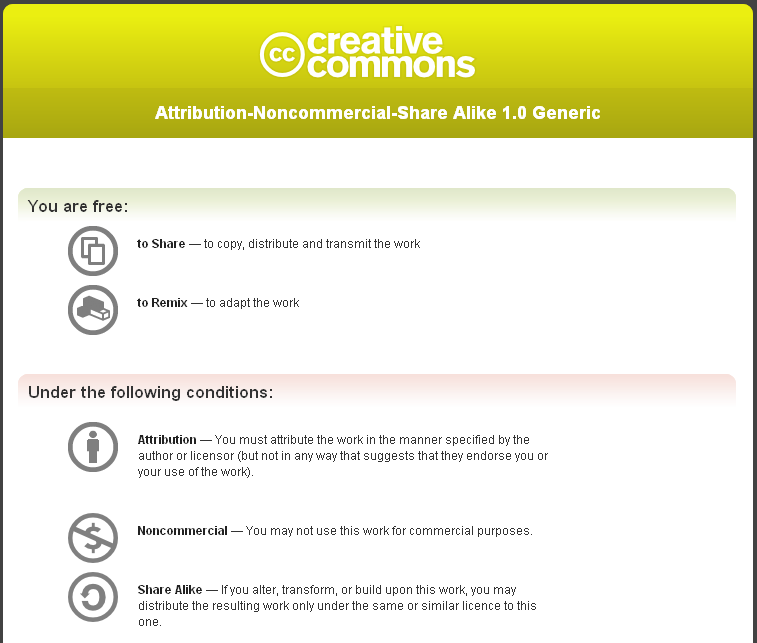
\includegraphics[width=0.74\textwidth]
		{assets/pics/creative_common.png}
	\caption{\license}
	\label{fig:lisensi}
\end{figure}

\pic~\ref{fig:lisensi} diambil dari 
\url{http://creativecommons.org/licenses/by-nc-sa/1.0/deed.en_CA}. 
Jika ingin mengentahui lebih lengkap mengenai \license, silahkan buka 
\url{http://creativecommons.org/licenses/by-nc-sa/1.0/legalcode}. 
Seluruh dokumen yang dibuat dengan menggunakan template ini sepenuhnya 
menjadi hak milik pembuat dokumen dan bebas didistribusikan sesuai dengan 
keperluan masing-masing. 
Lisensi hanya berlaku jika ada orang yang membuat template baru dengan 
menggunakan template ini sebagai dasarnya. 

Dokumen ini dibuat dengan \latex~juga. Untuk meyakinkan Anda, coba lihat 
properti dari dokumen ini dan Anda akan menemukan bagian seperti 
\pic~\ref{fig:pdflatex}. 
Dokumen ini dimaksudkan untuk memberikan gambaran kepada Anda seperti apa 
mudahnya menggunakan \latex~dan juga memperlihatkan betapa bagus dokumen 
yang dihasilkan. 
Seluruh url yang Anda temukan dapat Anda klik. 
Seluruh referensi yang ada juga dapat diklik. 
Untuk mengerti template yang disediakan, Anda tetap harus membuka kode 
\latex~dan bermain-main dengannya. 
Penjelasan dalam PDF ini masih bersifat gambaran dan tidak begitu 
mendetail, dapat dianggap sebagai pengantar singkat. 
Jika Anda merasa kesulitan dengan template ini, mungkin ada baiknya 
Anda belajar sedikit dasar-dasar \latex. 

\begin{figure}
	\centering
	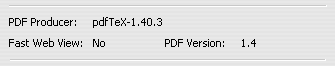
\includegraphics[width=0.54\textwidth]
		{assets/pics/mark.png}
	\caption{Dokumen Dibuat dengan PDFLatex}
	\label{fig:pdflatex}
\end{figure}

Semoga template ini dapat membantu orang-orang yang ingin mencoba menggunakan 
\latex. Semoga template ini juga tidak berhenti disini dengan ada kontribusi 
dari para penggunanya. 
Kami juga ingin berterima kasih kepada Andreas Febrian, Lia Sadita, Fahrurrozi 
Rahman, Andre Tampubolon, dan Erik Dominikus atas kontribusinya dalam template 
ini. 

\vspace*{0.1cm}
\begin{flushright}
Depok, 27 Februari 2019\\[0.1cm]
\vspace*{1cm}
\penulis

\end{flushright}
%
%
% \addChapter{LEMBAR PERSETUJUAN PUBLIKASI ILMIAH}
% % 
% @author  Andre Tampubolon, Andreas Febrian
% @version 1.01
% 

\chapter*{Halaman Pernyataan Persetujuan Publikasi Tugas Akhir untuk Kepentingan Akademis}

\vspace*{0.2cm}
\noindent 
Sebagai sivitas akademik Universitas Indonesia, saya yang bertanda 
tangan di bawah ini:
\vspace*{0.4cm}


\begin{tabular}{p{4.2cm} l p{6cm}}
	\bo{Nama} & : & \penulis \\ 	
	\bo{NPM} & : & \npm \\
	\bo{Program Studi} & : & \program\\	
	\bo{Fakultas} & : & \fakultas\\
	\bo{Jenis Karya} & : & \type \\
\end{tabular}

\vspace*{0.6cm}
\noindent demi pengembangan ilmu pengetahuan, menyetujui untuk memberikan 
kepada Universitas Indonesia \bo{Hak Bebas Royalti Noneksklusif 
(\textit{Non-exclusive Royalty Free Right})} atas karya ilmiah saya yang berjudul:
\begin{center}
	\judul
\end{center}
beserta perangkat yang ada (jika diperlukan). Dengan Hak Bebas Royalti 
Noneksklusif ini Universitas Indonesia berhak menyimpan, 
mengalihmedia/formatkan, mengelola dalam bentuk pangkalan data 
(\textit{database}), merawat, dan memublikasikan tugas akhir saya selama 
tetap mencantumkan nama saya sebagai penulis/pencipta dan sebagai 
pemilik Hak Cipta. \\

\noindent Demikian pernyatan ini saya buat dengan sebenarnya.

\begin{center}
	\vspace*{0.8cm}
	\begin{tabular}{rl}
		Dibuat di : & Depok \\
		Pada tanggal : & \tanggalPengesahan \\
	\end{tabular}\\

	\vspace*{0.2cm}
	Yang menyatakan \\
	\vspace*{1.1cm}
	(\penulis)
\end{center}

\newpage


%
% 
\addChapter{EXECUTIVE SUMMARY}
%
% Halaman Abstrak
%
% @author  Andreas Febrian
% @version 1.00
%

\chapter*{Executive Summary}

\vspace*{0.2cm}
{
% 	\setlength{\parindent}{0pt}
	
% 	\begin{tabular}{@{}l l p{10cm}}
% 		Nama&: & \penulis \\
% 		Program Studi&: & \program \\
% 		Judul&: & \judul \\
% 		Pembimbing&: & \pembimbing \\
% 	\end{tabular}

% 	\bigskip
% 	\bigskip

PT. XYZ saat ini menghadapi tantangan dalam pengelolaan jaringan yang melibatkan ratusan perangkat dengan kebutuhan konfigurasi yang berulang. Masalah utama muncul dari proses manual yang memerlukan banyak tenaga kerja dan waktu. Setiap perubahan konfigurasi jaringan harus dilakukan satu per satu, sehingga meningkatkan risiko kesalahan manusia (human error) dan memperlambat waktu penyelesaian. Selain itu, seiring dengan bertambahnya perangkat dan kompleksitas jaringan, PT. XYZ mengalami kendala dalam efisiensi operasional, yang akhirnya berdampak pada produktivitas tim dan kualitas layanan.

Untuk mengatasi masalah ini, PT. XYZ sedang mempertimbangkan implementasi Network Automation, yang diharapkan dapat menyederhanakan proses pengelolaan jaringan. Dengan otomatisasi, konfigurasi, monitoring, dan provisioning dapat dilakukan secara terpusat melalui dashboard tunggal. Hal ini akan mengurangi kebutuhan akan intervensi manual yang signifikan, mempercepat penyelesaian tugas, dan mengurangi potensi kesalahan.

Implementasi sistem network automation juga membawa berbagai keuntungan bisnis, baik yang terukur (tangible) maupun tidak terukur (intangible). Di antaranya adalah pengurangan biaya operasional karena berkurangnya intervensi manual, peningkatan efisiensi jaringan, pengurangan downtime, serta peningkatan skala operasional tanpa perlu menambah personel teknis. Dari sisi intangible, otomatisasi akan meningkatkan kualitas layanan, mempercepat inovasi, meningkatkan kepuasan pengguna, dan memperkuat ketahanan jaringan terhadap gangguan.

Namun, PT. XYZ juga menghadapi beberapa tantangan dalam implementasi ini. Kompleksitas infrastruktur jaringan yang terdiri dari berbagai vendor dan teknologi berbeda memerlukan solusi yang mendukung multi-vendor dan protokol terbuka. Selain itu, tim jaringan memerlukan peningkatan keterampilan dalam scripting, pemrograman, dan penggunaan API untuk mendukung transisi ke network automation.

Secara keseluruhan, otomatisasi jaringan di PT. XYZ diharapkan dapat meningkatkan efisiensi operasional, mengurangi biaya, dan memberikan layanan yang lebih stabil dan responsif, serta menyiapkan perusahaan untuk menghadapi pertumbuhan dan ekspansi di masa depan.

	\bigskip

% 	Kata kunci:\\
% 	Informasi, \textit{information literacy}, \textit{information skills}
}

\newpage
%
%
% %
% Halaman Abstract
%
% @author  Andreas Febrian
% @version 1.00
%

\chapter*{Abstract}

\vspace*{0.2cm}
{
	\setlength{\parindent}{0pt}
	
	\begin{tabular}{@{}l l p{10cm}}
		Name&: & \penulis \\
		Study Program&: & \program \\
		Title&: & \judulInggris \\
		Counsellor&: & \pembimbing \\
	\end{tabular}

	\bigskip
	\bigskip

	The focus of this study is the freshman student of Faculty of Psychology at University of
	Indonesia experience of acquiring, evaluating and using information, when they enroll in
	“Program Dasar Pendidikan Tinggi (PDPT)”. The purpose of this study is to understand
	how freshman students acquire, evaluate and use information. Knowing this will allow
	library to identify changes should be made to improve user education program at
	University of Indonesia. This research is qualitative descriptive interpretive. The data
	were collected by means of deep interview. The researcher suggests that library should
	improve the user education program and provide facilities which can help students to be
	information literate.

	\bigskip

	Key words:\\
	Information literacy, information skills, information
}

\newpage

%
% Daftar isi, gambar, dan tabel
%
\phantomsection
\tableofcontents
\clearpage
\phantomsection
\listoffigures
\clearpage
\phantomsection
\listoftables
\clearpage
\phantomsection
\listoflistings
\clearpage

%
% Gunakan penomeran Arab (1, 2, 3, ...) setelah bagian ini.
%
\pagenumbering{arabic}

%
%
%
%-----------------------------------------------------------------------------%
\chapter{\babSatu}
%-----------------------------------------------------------------------------%
% \todo{tambahkan kata-kata pengantar bab 1 disini}


% %-----------------------------------------------------------------------------%
% \section{Latar Belakang}
% %-----------------------------------------------------------------------------%
% \todo{tuliskan latar belakang penelitian disini}


% %-----------------------------------------------------------------------------%
% \section{Permasalahan}
% %-----------------------------------------------------------------------------%
% Pada bagian ini akan dijelaskan mengenai definisi permasalahan 
% yang \saya~hadapi dan ingin diselesaikan serta asumsi dan batasan 
% yang digunakan dalam menyelesaikannya.


% %-----------------------------------------------------------------------------%
% \subsection{Definisi Permasalahan}
% %-----------------------------------------------------------------------------%
% \todo{Tuliskan permasalahan yang ingin diselesaikan. Bisa juga
% 	berbentuk pertanyaan}


% %-----------------------------------------------------------------------------%
% \subsection{Batasan Permasalahan}
% %-----------------------------------------------------------------------------%
% \todo{Umumnya ada asumsi atau batasan yang digunakan untuk 
% 	menjawab pertanyaan-pertanyaan penelitian diatas.}


% %-----------------------------------------------------------------------------%
% \section{Tujuan}
% %-----------------------------------------------------------------------------%
% \todo{Tuliskan tujuan penelitian.}


% %-----------------------------------------------------------------------------%
% \section{Posisi Penelitian}
% %-----------------------------------------------------------------------------%
% \todo{Posisi penelitian Anda jika dilihat secara bersamaan dengan 
% 	peneliti-peneliti lainnya. Akan lebih baik lagi jika ikut menyertakan 
% 	diagram yang menjelaskan hubungan dan keterkaitan antar 
% 	penelitian-penelitian sebelumnya}


% %-----------------------------------------------------------------------------%
% \section{Metodologi Penelitian}
% %-----------------------------------------------------------------------------%
% \todo{Tuliskan metodologi penelitian yang digunakan.}


% %-----------------------------------------------------------------------------%
% \section{Sistematika Penulisan}
% %-----------------------------------------------------------------------------%
% Sistematika penulisan laporan adalah sebagai berikut:
% \begin{itemize}
% 	\item Bab 1 \babSatu \\
% 	\item Bab 2 \babDua \\
% 	\item Bab 3 \babTiga \\
% 	\item Bab 4 \babEmpat \\
% 	\item Bab 5 \babLima \\
% 	\item Bab 6 \babEnam \\
% 	\item Bab 7 \kesimpulan \\
% \end{itemize}

% \todo{Tambahkan penjelasan singkat mengenai isi masing-masing bab.}

\section{Project Sponsor}

\begin{table}[h!]
    \centering
    \caption{Project Sponsor}
    \begin{tabular}{|l|l|}
        \hline
        \textbf{Nama} & Haykal Rasidi \\ \hline
        \textbf{Jabatan} & IT Infrastruktur Manager \\ \hline
        \textbf{Kontak} & +62 813-8044-7624 \\ \hline
    \end{tabular}
\end{table}

\section{Business Needs}

Issue ini berawal dari keresahan beberapa karyawan network engineer di tempat saya bekerja dalam melakukan konfigurasi perintah/command yang berulang ke banyak perangkat. Untuk melakukan hal tersebut memerlukan beberapa engineer yang tujuannya agar pekerjaan yang dilakukan lebih cepat selesai. 

Permasalahan berikutnya jika perangkat yang akan dikonfigurasi semakin hari semakin bertambah dan konfigurasi perintah/command semakin panjang, maka engineer dan waktu yang dibutuhkan untuk menyelesaikan proses tersebut juga semakin bertambah.  

Permasalahan lain, faktor human error akan semakin besar dalam melakukan konfigurasi yang berulang dan ke banyak perangkat. 

Oleh karena itu perlu adanya system yang mampu menyederhanakan proses tersebut agar menjadi efektif dan lebih efisien. 


\newpage 

\begin{table}[h!]
    \caption{Harapan, Kenyataan, Masalah}
    \begin{longtable}{|p{4cm}|p{4cm}|>{\raggedright\arraybackslash}p{3.5cm}|}
        \hline
        \textbf{Harapan} & \textbf{Kenyataan} & \textbf{Masalah} \\
        \hline
        Tidak memerlukan sumber daya manusia yang terlalu banyak dalam melakukan konfigurasi ke banyak perangkat. &
        Saat ini dalam melakukan konfigurasi ke banyak perangkat diperlukan beberapa sumber daya manusia. &
        \multirow{4}{\linewidth}{%
            \raggedright
            Diperlukan suatu sistem informasi yang mampu mengintegrasikan seluruh perangkat dalam satu dashboard untuk melakukan konfigurasi perintah/command secara bersamaan dalam satu waktu.
        } \\
        \cline{1-2}
        Tidak memerlukan waktu yang terlalu lama dalam melakukan banyak proses ke banyak perangkat. &
        Saat ini waktu yang dibutuhkan akan bertambah jika perangkat dan konfigurasi yang dilakukan semakin banyak. & \\
        \cline{1-2}
        Mengurangi human error dalam melakukan konfigurasi yang panjang ke banyak perangkat dalam waktu yang singkat. &
        Sering terjadi kesalahan dalam melakukan konfigurasi perintah/command atau ada step yang terlewat. & \\
        \cline{1-2}
        Sistem yang mengintegrasikan banyak perangkat dalam satu dashboard untuk memudahkan dalam manajemen konfigurasi. &
        Belum ada sistem yang mengintegrasikan, saat ini dalam melakukan konfigurasi dilakukan satu persatu dengan membuka akses terhadap tiap perangkat. & \\
        \hline
    \end{longtable}
\end{table}

Network Automation menjadi sebuah solusi atas beberapa permasalahan tersebut, mulai dari biaya yang tinggi untuk hire beberapa sumber daya untuk melakukan pekerjaan tersebut, menyederhanakan sebuah proses yang kompleks dan panjang hingga menghindari banyaknya kesalahan dalam melakukan konfigurasi. Network automation sebuah solusi yang diimplementasikan dalam bentuk sistem yang akan menunjang suatu proses bisnis perusahaan dari sisi IT infrastruktur.

\begin{figure}
	\centering
	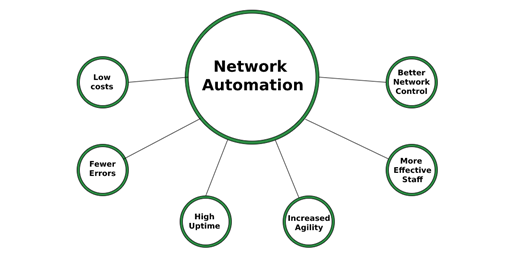
\includegraphics[width=0.70\textwidth]{assets/pics/network_automation.png}
	\caption{Network Automation}
	\label{fig:NetworkAutomation}
\end{figure}


\subsection{Non-Functional Requirements (NFR)}
\begin{enumerate}
    \item \textbf{Scalability (Skalabilitas)}: Kemampuan sistem untuk menangani peningkatan jumlah perangkat jaringan.
    
    \item \textbf{Performance (Kinerja)}
    \begin{itemize}
        \item Latency rendah dalam pengiriman konfigurasi atau perubahan jaringan.
        \item Sistem otomatisasi harus dapat menangani volume besar tugas-tugas konfigurasi secara bersamaan.
    \end{itemize}
    
    \item \textbf{Security (Keamanan)}
    \begin{itemize}
        \item Proses otomatisasi harus mematuhi standar keamanan yang tinggi untuk mencegah akses tidak sah atau modifikasi pada konfigurasi jaringan.
        \item Enkripsi data: Semua data yang dikirimkan melalui jaringan dan proses otomatisasi harus terenkripsi.
        \item Authentication \& Authorization: Sistem harus memastikan hanya pengguna yang sah dapat menjalankan tugas otomatisasi dan harus ada kontrol akses yang ketat.
    \end{itemize}
    
    \item \textbf{Usability (Kemudahan Penggunaan)}
    \begin{itemize}
        \item Dashboard otomatisasi jaringan harus intuitif dan mudah digunakan oleh admin jaringan tanpa membutuhkan pelatihan yang terlalu intensif.
        \item Error handling yang jelas: Pesan kesalahan dan status operasional harus mudah dipahami oleh pengguna.
    \end{itemize}
    
    \item \textbf{Interoperability (Interoperabilitas)}
    \begin{itemize}
        \item Sistem otomatisasi harus dapat berfungsi dengan baik di berbagai perangkat dan vendor jaringan yang berbeda.
        \item Standar terbuka: Memastikan kompatibilitas dengan berbagai protokol jaringan dan perangkat keras yang digunakan.
    \end{itemize}
    
    \item \textbf{Availability (Ketersediaan)}
    \begin{itemize}
        \item Sistem otomatisasi harus selalu tersedia untuk digunakan kapan saja.
        \item High availability (Ketersediaan tinggi): Sistem harus memiliki redundansi untuk menghindari downtime.
    \end{itemize}
    
    \item \textbf{Auditability (Kemampuan Audit)}: Sistem harus mendukung kemampuan untuk melacak semua perubahan konfigurasi jaringan dan menyediakan log atau laporan audit yang komprehensif.
    
    \item \textbf{Flexibility (Fleksibilitas)}: Kemampuan sistem untuk beradaptasi dengan kebutuhan yang terus berubah dan berkembang, termasuk mendukung teknologi baru atau perubahan dalam arsitektur jaringan.
\end{enumerate}

Secara umum, fungsi non-fungsional dalam network automation menekankan aspek kualitas sistem yang berkaitan dengan bagaimana sistem beroperasi, bukan hanya apa yang dapat dilakukan oleh sistem tersebut.

\subsection{Functional Requirements}
\begin{enumerate}
    \item \textbf{Pengelolaan Konfigurasi (Configuration Management)}
    \begin{itemize}
        \item Membuat, menyimpan, dan menerapkan perubahan konfigurasi perangkat jaringan secara otomatis.
        \item Melakukan backup dan restore konfigurasi perangkat jaringan.
    \end{itemize}
    
    \item \textbf{Orkestrasi Jaringan}
    \begin{itemize}
        \item Mengkoordinasikan beberapa proses otomatisasi sekaligus di berbagai perangkat atau segmen jaringan.
        \item Integrasi dengan berbagai platform atau perangkat lunak jaringan yang berbeda, sehingga seluruh infrastruktur jaringan dapat diatur secara konsisten.
    \end{itemize}
    
    \item \textbf{Integrasi dengan Sistem Manajemen Jaringan Lain}
    \begin{itemize}
        \item Berfungsi sebagai penghubung dengan alat manajemen jaringan lainnya seperti SDN (Software Defined Networking), NFV (Network Functions Virtualization), dan platform monitoring untuk orkestrasi yang lebih luas.
    \end{itemize}
\end{enumerate}

Fungsi-fungsi tersebut berfokus pada bagaimana otomatisasi jaringan dapat membantu administrator jaringan mengelola infrastruktur secara efisien, mengurangi kesalahan manual, meningkatkan kecepatan, serta memastikan stabilitas dan keamanan.

\section{Business Value}

\subsection{Tangible Business Value (Nilai Bisnis yang Terukur/Terlihat)}
\begin{itemize}
    \item \textbf{Pengurangan Biaya Operasional}: Otomasi jaringan mengurangi kebutuhan akan intervensi manual, sehingga menghemat biaya tenaga kerja dan mempercepat penyelesaian tugas operasional.
    \item \textbf{Efisiensi Jaringan}: Dengan proses otomatisasi, jaringan dapat dioptimalkan secara efisien, sehingga meningkatkan pemanfaatan sumber daya jaringan dan mengurangi biaya infrastruktur.
    \item \textbf{Pengurangan Waktu Downtime}: Network automation memungkinkan deteksi dan perbaikan masalah lebih cepat, yang berarti waktu downtime jaringan berkurang, meningkatkan produktivitas.
    \item \textbf{Peningkatan Skala (Scalability)}: Otomasi memungkinkan perusahaan mengelola jaringan yang lebih besar tanpa perlu menambah jumlah personel teknis, sehingga memberikan skala yang lebih baik untuk ekspansi bisnis.
    \item \textbf{Kecepatan Implementasi}: Penerapan layanan dan konfigurasi jaringan menjadi lebih cepat dan akurat, yang memungkinkan perusahaan merespons kebutuhan bisnis dengan lebih cepat.
\end{itemize}

\subsection{Intangible Business Value (Nilai Bisnis yang Tidak Terlihat/Tidak Terukur Langsung)}
\begin{itemize}
    \item \textbf{Peningkatan Kualitas Layanan}: Dengan otomatisasi, perusahaan dapat memberikan layanan yang lebih stabil, minim gangguan, dan lebih responsif terhadap kebutuhan pelanggan.
    \item \textbf{Inovasi Lebih Cepat}: Otomasi jaringan membebaskan waktu dan sumber daya tim TI untuk fokus pada inovasi dan peningkatan layanan daripada tugas-tugas rutin.
    \item \textbf{Peningkatan Kepuasan}: Ketersediaan jaringan yang lebih baik dan peningkatan responsivitas layanan meningkatkan pengalaman pengguna, yang berkontribusi pada kepuasan pelanggan.
    \item \textbf{Ketahanan (Resilience)}: Otomasi membantu membangun jaringan yang lebih tangguh terhadap perubahan dan kegagalan, sehingga bisnis dapat terus berjalan dengan gangguan minimal.
\end{itemize}

\section{Special Issues}
\begin{enumerate}
    \item \textbf{Kompleksitas Infrastruktur yang Beragam}: Jaringan modern sering kali terdiri dari berbagai perangkat keras, vendor, dan teknologi yang berbeda (misalnya router, switch, firewall dari berbagai merek). Masing-masing perangkat mungkin memiliki protokol dan API yang berbeda untuk diotomatisasi, sehingga menyulitkan pengelolaan dengan satu solusi universal.
    
    \item \textbf{Keamanan (Security)}: Otomatisasi jaringan dapat meningkatkan risiko jika tidak dikelola dengan baik. Skrip otomatisasi yang salah atau memiliki kerentanan dapat membuka celah bagi penyerang.
    
    \item \textbf{Skalabilitas}: Ketika jaringan tumbuh besar dan kompleks, alat otomasi harus mampu menyesuaikan dan berfungsi dengan baik di lingkungan besar. Masalah skalabilitas ini dapat mencakup performa alat otomasi, manajemen database, atau integrasi dengan sistem lain.
    
    \item \textbf{Pengelolaan Perubahan (Change Management)}: Proses otomatisasi dapat menyebabkan perubahan di jaringan dengan cepat dan dalam skala besar. Jika tidak dikelola dengan baik, perubahan yang tidak diverifikasi bisa merusak konfigurasi dan menyebabkan downtime.
    
    \item \textbf{Kurangnya Standardisasi}: Tidak semua vendor atau organisasi menggunakan standar yang sama dalam mengimplementasikan jaringan. Hal ini menciptakan tantangan dalam mengintegrasikan alat otomatisasi.
    
    \item \textbf{Kebutuhan Skill yang Khusus}: Mengimplementasikan otomatisasi jaringan memerlukan keterampilan baru bagi tim jaringan, seperti pemrograman, pemahaman API, dan penguasaan alat otomasi. Tim jaringan tradisional mungkin perlu waktu untuk menyesuaikan diri dengan teknologi baru ini.
    
    \item \textbf{Kendala Kompatibilitas dengan Teknologi Lama (Legacy Systems)}: Banyak jaringan masih menggunakan perangkat atau sistem lama yang tidak mendukung otomatisasi modern, sehingga sulit untuk mengintegrasikannya ke dalam proses otomatisasi.
\end{enumerate}




%-----------------------------------------------------------------------------%
\chapter{\babDua}
%-----------------------------------------------------------------------------%
\todo{tambahkan kata-kata pengantar bab 2 disini}

%-----------------------------------------------------------------------------%
\section{\latex~Secara Singkat}
%-----------------------------------------------------------------------------%
Definisi dari LaTeX \citep{lankton2008introduction} adalah: \\ 
\begin{tabular}{| p{13cm} |}
	\hline 
	\\
	LaTeX is a family of programs designed to produce publication-quality 
	typeset documents. It is particularly strong when working with 
	mathematical symbols. \\	
	The history of LaTeX begins with a program called TEX. In 1978, a 
	computer scientist by the name of Donald Knuth grew frustrated with the 
	mistakes that his publishers made in typesetting his work. He decided 
	to create a typesetting program that everyone could easily use to 
	typeset documents, particularly those that include formulae, and made 
	it freely available. The result is TEX. \\	
	Knuth's product is an immensely powerful program, but one that does 
	focus very much on small details. A mathematician and computer 
	scientist by the name of Leslie Lamport wrote a variant of TEX called 
	LaTeX that focuses on document structure rather than such details. \\
	\\
	\hline
\end{tabular}

\vspace*{0.8cm}

Contoh sitasi lainnya menggunakan \verb|\citep| adalah saat kita mau mensitasi pekerjaan tentang \textit{machine learning} \citep{chin2000learning} dan \textit{dynamic programming} \citep{barto1995learning}. \\

Dokumen \latex~sangat mudah, seperti halnya membuat dokumen teks biasa. Ada 
beberapa perintah yang diawali dengan tanda '\bslash'. 
Seperti perintah \bslash\bslash~yang digunakan untuk memberi baris baru. 
Perintah tersebut juga sama dengan perintah \bslash newline. 
Pada bagian ini akan sedikit dijelaskan cara manipulasi teks dan 
perintah-perintah \latex~yang mungkin akan sering digunakan. 
Jika ingin belajar hal-hal dasar mengenai \latex, silahkan kunjungi: 

\begin{itemize}
	\item \url{http://frodo.elon.edu/tutorial/tutorial/}, atau
	\item \url{http://www.maths.tcd.ie/~dwilkins/LaTeXPrimer/}
\end{itemize}


%-----------------------------------------------------------------------------%
\section{\latex~Kompiler dan IDE}
%-----------------------------------------------------------------------------%
Agar dapat menggunakan \latex~(pada konteks hanya sebagai pengguna), Anda 
tidak perlu banyak tahu mengenai hal-hal didalamnya. 
Seperti halnya pembuatan dokumen secara visual (contohnya Open Office (OO) 
Writer), Anda dapat menggunakan \latex~dengan cara yang sama. 
Orang-orang yang menggunakan \latex~relatif lebih teliti dan terstruktur 
mengenai cara penulisan yang dia gunakan, \latex~memaksa Anda untuk seperti 
itu.  

Kembali pada bahasan utama, untuk mencoba \latex~Anda cukup mendownload 
kompiler dan IDE. Saya menyarankan menggunakan Texlive dan Texmaker. 
Texlive dapat didownload dari \url{http://www.tug.org/texlive/}. 
Sedangkan Texmaker dapat didownload dari 
\url{http://www.xm1math.net/texmaker/}. 
Untuk pertama kali, coba buka berkas thesis.tex dalam template yang Anda miliki 
pada Texmaker. 
Dokumen ini adalah dokumen utama. 
Tekan F6 (PDFLaTeX) dan Texmaker akan mengkompilasi berkas tersebut menjadi 
berkas PDF. 
Jika tidak bisa, pastikan Anda sudah menginstall Texlive. 
Buka berkas tersebut dengan menekan F7. 
Hasilnya adalah sebuah dokumen yang sama seperti dokumen yang Anda baca saat 
ini. 


%-----------------------------------------------------------------------------%
\section{Bold, Italic, dan Underline}
%-----------------------------------------------------------------------------%
Hal pertama yang mungkin ditanyakan adalah bagaimana membuat huruf tercetak 
tebal, miring, atau memiliki garis bawah. 
Pada Texmaker, Anda bisa melakukan hal ini seperti halnya saat mengubah dokumen 
dengan OO Writer. 
Namun jika tetap masih tertarik dengan cara lain, ini dia: 

\begin{itemize}
	\item \bo{Bold} \\
		Gunakan perintah \bslash textbf$\lbrace\rbrace$ atau 
		\bslash bo$\lbrace\rbrace$. 
	\item \f{Italic} \\
		Gunakan perintah \bslash textit$\lbrace\rbrace$ atau 
		\bslash f$\lbrace\rbrace$. 
	\item \underline{Underline} \\
		Gunakan perintah \bslash underline$\lbrace\rbrace$.
	\item $\overline{Overline}$ \\
		Gunakan perintah \bslash overline. 
	\item $^{superscript}$ \\
		Gunakan perintah \bslash $\lbrace\rbrace$. 
	\item $_{subscript}$ \\
		Gunakan perintah \bslash \_$\lbrace\rbrace$. 
\end{itemize}

Perintah \bslash f dan \bslash bo hanya dapat digunakan jika package 
uithesis digunakan. 


%-----------------------------------------------------------------------------%
\section{Memasukan Gambar}
%-----------------------------------------------------------------------------%
Setiap gambar dapat diberikan caption dan diberikan label. Label dapat 
digunakan untuk menunjuk gambar tertentu. 
Jika posisi gambar berubah, maka nomor gambar juga akan diubah secara 
otomatis. 
Begitu juga dengan seluruh referensi yang menunjuk pada gambar tersebut. 
Contoh sederhana adalah \pic~\ref{fig:testGambar}. 
Silahkan lihat code \latex~dengan nama bab2.tex untuk melihat kode lengkapnya. 
Harap diingat bahwa caption untuk gambar selalu terletak dibawah gambar. 

\begin{figure}
	\centering
	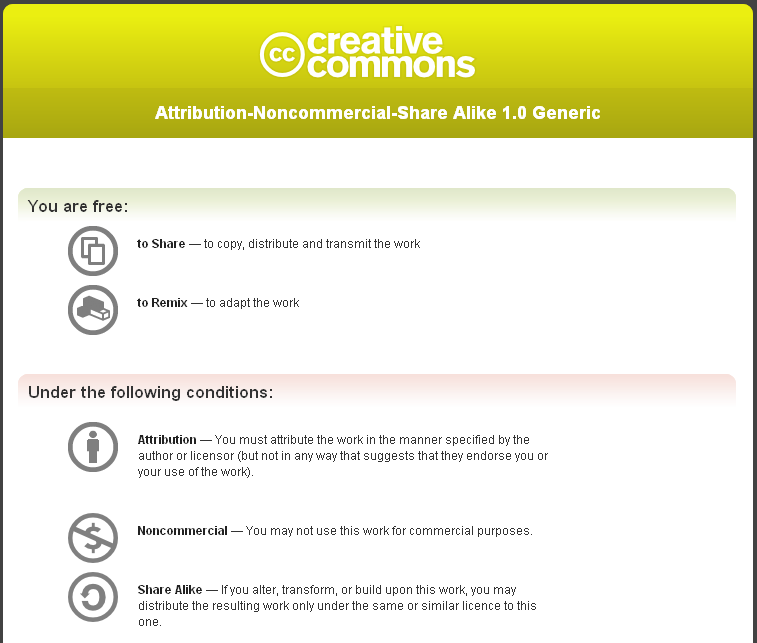
\includegraphics[width=0.50\textwidth]
		{assets/pics/creative_common.png}
	\caption{\license.}
	\label{fig:testGambar}
\end{figure}


%-----------------------------------------------------------------------------%
\section{Membuat Tabel}
%-----------------------------------------------------------------------------%
Seperti pada gambar, tabel juga dapat diberi label dan caption. 
Caption pada tabel terletak pada bagian atas tabel. 
Contoh tabel sederhana dapat dilihat pada \tab~\ref{tab:tab1}.

\begin{table}
	\centering
	\caption{Contoh Tabel}
	\label{tab:tab1}
	\begin{tabular}{| l | c r |}
		\hline
		& kol 1 & kol 2 \\ 
		\hline
		baris 1 & 1 & 2 \\
		baris 2 & 3 & 4 \\
		baris 3 & 5 & 6 \\
		jumlah  & 9 & 12 \\
		\hline
	\end{tabular}
\end{table}

Ada jenis tabel lain yang dapat dibuat dengan \latex~berikut 
beberapa diantaranya. 
Contoh-contoh ini bersumber dari 
\url{http://en.wikibooks.org/wiki/LaTeX/Tables}

\begin{table}
	\centering
	\caption{An Example of Rows Spanning Multiple Columns}
	\label{row.spanning}
	\begin{tabular}{|l|l|*{6}{c|}}
  		\hline % create horizontal line
  		No & Name & \multicolumn{3}{|c|}{Week 1} & \multicolumn{3}{|c|}{Week 2} \\
  		\cline{3-8} % create line from 3rd column till 8th column
  		& & A & B & C & A & B & C\\
  		\hline
  		1 & Lala & 1 & 2 & 3 & 4 & 5 & 6\\
  		2 & Lili & 1 & 2 & 3 & 4 & 5 & 6\\
  		3 & Lulu & 1 & 2 & 3 & 4 & 5 & 6\\
  		\hline
	\end{tabular}
\end{table}

\begin{table}
	\centering
	\caption{An Example of Columns Spanning Multiple Rows}
	\label{column.spanning}
	\begin{tabular}{|l|c|l|}
		\hline
		Percobaan & Iterasi & Waktu \\
		\hline
		Pertama & 1 & 0.1 sec \\ \hline
		\multirow{2}{*}{Kedua} & 1 & 0.1 sec \\
 		& 3 & 0.15 sec \\ 
 		\hline
		\multirow{3}{*}{Ketiga} & 1 & 0.09 sec \\
 		& 2 & 0.16 sec \\
 		& 3 & 0.21 sec \\ 
 		\hline
	\end{tabular}
\end{table}

\begin{table}
	\centering
	\caption{An Example of Spanning in Both Directions Simultaneously}
	\label{mix.spanning}
	\begin{tabular}{cc|c|c|c|c|}
		\cline{3-6}
		& & \multicolumn{4}{|c|}{Title} \\ \cline{3-6}
		& & A & B & C & D \\ \hline
		\multicolumn{1}{|c|}{\multirow{2}{*}{Type}} &
		\multicolumn{1}{|c|}{X} & 1 & 2 & 3 & 4\\ \cline{2-6}
		\multicolumn{1}{|c|}{}                        &
		\multicolumn{1}{|c|}{Y} & 0.5 & 1.0 & 1.5 & 2.0\\ \cline{1-6}
		\multicolumn{1}{|c|}{\multirow{2}{*}{Resource}} &
		\multicolumn{1}{|c|}{I} & 10 & 20 & 30 & 40\\ \cline{2-6}
		\multicolumn{1}{|c|}{}                        &
		\multicolumn{1}{|c|}{J} & 5 & 10 & 15 & 20\\ \cline{1-6}
	\end{tabular}
\end{table}


%-----------------------------------------------------------------------------%
\chapter{\babTiga}
%-----------------------------------------------------------------------------%
\todo{tambahkan kata-kata pengantar bab 1 disini}


%-----------------------------------------------------------------------------%
\section{Satu Persamaan}
%-----------------------------------------------------------------------------%

\noindent \begin{align}\label{eq:garis}
	\cfrac{y - y_{1}}{y_{2} - y_{1}} = 
	\cfrac{x - x_{1}}{x_{2} - x_{1}}
\end{align}

\equ~\ref{eq:garis} diatas adalah persamaan garis. 
\equ~\ref{eq:garis} dan \ref{eq:bola} sama-sama dibuat dengan perintah \bslash
align. 
Perintah ini juga dapat digunakan untuk menulis lebih dari satu persamaan. 

\noindent \begin{align}\label{eq:bola}
	\underbrace{|\overline{ab}|}_{\text{pada bola $|\overline{ab}| = r$}} 
		= \sqrt[2]{(x_{b} - x_{a})^{2} + (y_{b} - y_{a})^{2} + 
				\vert\vert(z_{b} - z_{a})^{2}}
\end{align}

%-----------------------------------------------------------------------------%
\section{Lebih dari Satu Persamaan}
\label{sec:multiEqu}
%-----------------------------------------------------------------------------%
\noindent \begin{align}\label{eq:matriks}	
	|\overline{a} * \overline{b}| &= |\overline{a}| |\overline{b}| \sin\theta 
		\\[0.2cm]
	\overline{a} * \overline{b} &=  
		\begin{array}{| c c c |}
			\hat{i} & x_{1} & x_{2} \\
			\hat{j} & y_{1} & y_{2} \\
			\hat{k} & z_{1} & z_{2} \\
		\end{array} \nonumber \\[0.2cm]
	&= \hat{i} \,
		\begin{array}{ | c c | }
			y_{1} & y_{2} \\
			z_{1} & z_{2} \\
		\end{array} 
	   + \hat{j} \,
		\begin{array}{ | c c | }
			z_{1} & z_{2} \\
			x_{1} & x_{2} \\
		\end{array} 
	   + \hat{k} \,	
		\begin{array}{ | c c | }
			x_{1} & x_{2} \\
			y_{1} & y_{2} \\
		\end{array}
		\nonumber
\end{align}

Pada \equ~\ref{eq:matriks} dapat dilihat beberapa baris menjadi satu bagian 
dari \equ~\ref{eq:matriks}. 
Sedangkan dibawah ini dapat dilihat bahwa dengan cara yang sama, \equ~
\ref{eq:gabungan1}, \ref{eq:gabungan2}, dan \ref{eq:gabungan3} memiliki nomor 
persamaannya masing-masing. 

\noindent \begin{align}\label{eq:gabungan1}	
	\int_{a}^{b} f(x)\, dx + \int_{b}^{c} f(x) \, dx = \int_{a}^{c} f(x) \, dx
		\\\label{eq:gabungan2}
	\lim_{x \to \infty} \frac{f(x)}{g(x)} = 0 \hspace{1cm} 
		\text{jika pangkat $f(x)$ $<$ pangkat $g(x)$} \\\label{eq:gabungan3}
	a^{m^{a \, ^{n}\log b }} = b^{\frac{m}{n}}
\end{align}


%-----------------------------------------------------------------------------%
\chapter{\babEmpat}
%-----------------------------------------------------------------------------%
% \todo{tambahkan kata-kata pengantar bab 1 disini}

% %-----------------------------------------------------------------------------%
% \section{thesis.tex}
% %-----------------------------------------------------------------------------%
% Berkas ini berisi seluruh berkas Latex yang dibaca, jadi bisa dikatakan sebagai 
% berkas utama. Dari berkas ini kita dapat mengatur bab apa saja yang ingin 
% kita tampilkan dalam dokumen.


% %-----------------------------------------------------------------------------%
% \section{laporan\_setting.tex}
% %-----------------------------------------------------------------------------%
% Berkas ini berguna untuk mempermudah pembuatan beberapa template standar. 
% Anda diminta untuk menuliskan judul laporan, nama, npm, dan hal-hal lain yang 
% dibutuhkan untuk pembuatan template. 


% %-----------------------------------------------------------------------------%
% \section{istilah.tex}
% %-----------------------------------------------------------------------------%
% Berkas istilah digunakan untuk mencatat istilah-istilah yang digunakan. 
% Fungsinya hanya untuk memudahkan penulisan.
% Pada beberapa kasus, ada kata-kata yang harus selalu muncul dengan tercetak 
% miring atau tercetak tebal. 
% Dengan menjadikan kata-kata tersebut sebagai sebuah perintah \latex~tentu akan 
% mempercepat dan mempermudah pengerjaan laporan. 


% %-----------------------------------------------------------------------------%
% \section{hype.indonesia.tex}
% %-----------------------------------------------------------------------------%
% Berkas ini berisi cara pemenggalan beberapa kata dalam bahasa Indonesia. 
% \latex~memiliki algoritma untuk memenggal kata-kata sendiri, namun untuk 
% beberapa kasus algoritma ini memenggal dengan cara yang salah. 
% Untuk memperbaiki pemenggalan yang salah inilah cara pemenggalan yang benar 
% ditulis dalam berkas hype.indonesia.tex.


% %-----------------------------------------------------------------------------%
% \section{pustaka.tex}
% %-----------------------------------------------------------------------------%
% Berkas pustaka.tex berisi seluruh daftar referensi yang digunakan dalam 
% laporan. 
% Anda bisa membuat model daftar referensi lain dengan menggunakan bibtex.
% Untuk mempelajari bibtex lebih lanjut, silahkan buka 
% \url{http://www.bibtex.org/Format}. 
% Untuk merujuk pada salah satu referensi yang ada, gunakan perintah \bslash 
% cite, e.g. \bslash cite\{lankton2008introduction\} yang akan akan memunculkan 
% \cite{lankton2008introduction}


% %-----------------------------------------------------------------------------%
% \section{bab[1 - 6].tex}
% %-----------------------------------------------------------------------------%
% Berkas ini berisi isi laporan yang Anda tulis. 
% Setiap nama berkas e.g. bab1.tex merepresentasikan bab dimana tulisan tersebut 
% akan muncul. 
% Sebagai contoh, kode dimana tulisan ini dibaut berada dalam berkas dengan nama 
% bab4.tex. 
% Ada enam buah berkas yang telah disiapkan untuk mengakomodir enam bab dari 
% laporan Anda, diluar bab kesimpulan dan saran. 
% Jika Anda tidak membutuhkan sebanyak itu, silahkan hapus kode dalam berkas 
% thesis.tex yang memasukan berkas \latex~yang tidak dibutuhkan;  contohnya 
% perintah \bslash include\{bab6.tex\} merupakan kode untuk memasukan berkas 
% bab6.tex kedalam laporan.

% %-----------------------------------------------------------------------------%
% \section{Penulisan \textit{code} atau \textit{pseudocode} program}
% %-----------------------------------------------------------------------------%

% \subsection{\textit{Inline}}

% Dengan perintah \verb|\verb|: \verb|System.out.println("Hello, World");| \\
% Dengan perintah \textit{custom} \verb|\code|: \code{System.out.println("Hello, World"); }
% Dengan perintah \verb|\mintinline|: \mintinline{java}{System.out.println("Hello, World"); }

% \subsection{\textit{Multiline}}

% Dengan perintah \verb|verbatim|: 

% \begin{verbatim}	
% public class HelloWorld {
%     public static void main(String[] args) {
%         // Prints "Hello, World" to the terminal window.
%         System.out.println("Hello, World");
%     }
% }
% \end{verbatim}

% Dengan perintah \verb|minted|: Kode \ref{code:hw:minted}
% \begin{listing}[H]
%     \begin{minted}{python}
% def binary_accuracy(y_true, y_pred):
%     return K.mean(K.equal(y_true, K.round(y_pred)), axis=-1)


% def categorical_accuracy(y_true, y_pred):
%     return K.cast(K.equal(K.argmax(y_true, axis=-1),
%                           K.argmax(y_pred, axis=-1)),
%                   K.floatx())


% def sparse_categorical_accuracy(y_true, y_pred):
%     # reshape in case it's in shape (num_samples, 1) instead of (num_samples,)
%     if K.ndim(y_true) == K.ndim(y_pred):
%         y_true = K.squeeze(y_true, -1)
%     # convert dense predictions to labels
%     y_pred_labels = K.argmax(y_pred, axis=-1)
%     y_pred_labels = K.cast(y_pred_labels, K.floatx())
%     return K.cast(K.equal(y_true, y_pred_labels), K.floatx())


% def top_k_categorical_accuracy(y_true, y_pred, k=5):
%     return K.mean(K.in_top_k(y_pred, K.argmax(y_true, axis=-1), k), axis=-1)


% def sparse_top_k_categorical_accuracy(y_true, y_pred, k=5):
%     # If the shape of y_true is (num_samples, 1), flatten to (num_samples,)
%     return K.mean(K.in_top_k(y_pred, K.cast(K.flatten(y_true), 'int32'), k),
%                   axis=-1)
%     \end{minted}
%     \caption{An excerpt from keras: \url{https://github.com/keras-team/keras/blob/master/keras/metrics.py}}
%     \label{code:hw:minted}
% \end{listing}

% Konfigurasi tampilan bisa dilakukan di \verb|uithesis.sty| dengan referensi dokumentasi di \url{https://github.com/gpoore/minted/blob/master/source/minted.pdf}


\section{Functional Requirement}

\todo{fill this}

\section{Non Functional Requirement}

\todo{fill this, requirement seperti operasional, performa, keamanan}




%-----------------------------------------------------------------------------%
\chapter{\babLima}
%-----------------------------------------------------------------------------%
\todo{Tambahkan kata-kata pengantar bab 5 disini.}


%-----------------------------------------------------------------------------%
\section{Mengubah Tampilan Teks}
%-----------------------------------------------------------------------------%
Beberapa perintah yang dapat digunakan untuk mengubah tampilan adalah: 
\begin{itemize}
	\item \bslash f \\
		Merupakan alias untuk perintah \bslash textit, contoh 
		\f{contoh hasil tulisan}.
	\item \bslash bi \\
		\bi{Contoh hasil tulisan}.
	\item \bslash bo \\
		\bo{Contoh hasil tulisan}.
	\item \bslash m \\
		Contoh\ hasil\ tulisan: $\alpha \not= \m{\alpha}$
	\item \bslash code \\ 
		\code{Contoh hasil tulisan}.
\end{itemize}


%-----------------------------------------------------------------------------%
\section{Memberikan Catatan}
%-----------------------------------------------------------------------------%
Ada dua perintah untuk memberikan catatan penulisan dalam dokumen yang Anda 
kerjakan, yaitu: 
\begin{itemize}
	\item \bslash todo \\
		Contoh: \\ \todo{Contoh bentuk todo.}
	\item \bslash todoCite \\ 
		Contoh: \todoCite
\end{itemize}


%-----------------------------------------------------------------------------%
\section{Menambah Isi Daftar Isi}
%-----------------------------------------------------------------------------%
Terkadang ada kebutuhan untuk memasukan kata-kata tertentu kedalam Daftar Isi. 
Perintah \bslash addChapter dapat digunakan untuk judul bab dalam Daftar isi. 
Contohnya dapat dilihat pada berkas thesis.tex.


%-----------------------------------------------------------------------------%
\section{Memasukan PDF}
%-----------------------------------------------------------------------------%
Untuk memasukan PDF dapat menggunakan perintah \bslash inpdf yang menerima satu 
buah argumen. Argumen ini berisi nama berkas yang akan digabungkan dalam 
laporan. PDF yang dimasukan degnan cara ini akan memiliki header dan footer 
seperti pada halaman lainnya. 

\inpdf{assets/pdfs/include}

Cara lain untuk memasukan PDF adalah dengan menggunakan perintah \bslash putpdf 
dengan satu argumen yang berisi nama berkas pdf. Berbeda dengan perintah 
sebelumnya, PDF yang dimasukan dengan cara ini tidak akan memiliki footer atau 
header seperti pada halaman lainnya. 

\putpdf{assets/pdfs/include}


%-----------------------------------------------------------------------------%
\section{Membuat Perintah Baru}
%-----------------------------------------------------------------------------%
Ada dua perintah yang dapat digunakan untuk membuat perintah baru, yaitu: 
\begin{itemize}
	\item \bslash Var \\
		Digunakan untuk membuat perintah baru, namun setiap kata yang diberikan
		akan diproses dahulu menjadi huruf kapital. 
		Contoh jika perintahnya adalah \bslash Var\{adalah\} makan ketika 
		perintah \bslash Var dipanggil, yang akan muncul adalah ADALAH. 
	\item \bslash var \\
		Digunakan untuk membuat perintah atau baru. 
\end{itemize}


%-----------------------------------------------------------------------------%
\chapter{\babEnam}
%-----------------------------------------------------------------------------%
\todo{tambahkan kata-kata pengantar bab 6 disini}


%-----------------------------------------------------------------------------%
\chapter{\babTujuh}
%-----------------------------------------------------------------------------%
\todo{fill this}

\section{Class Diagram}

\section{CRC Card}


%-----------------------------------------------------------------------------%
\chapter{\babDelapan}
%-----------------------------------------------------------------------------%
\todo{fill this}

\section{Use scenarios}

\section{Real Usecases}

\section{Behavorial State Machine Diagram}

\section{CRUDE Analysis}


%-----------------------------------------------------------------------------%
\chapter{\babSembilan}
%-----------------------------------------------------------------------------%

\todo{from this point onward its tugas 4 territory}

\section{Use Scenarios}

\section{Real Usecases}

\section{User Interfaces}

\subsection{Site Map}

\subsection{Windows Navigation Design}

\subsection{System Design Mockup}





%-----------------------------------------------------------------------------%
\chapter{\babSepuluh}
%-----------------------------------------------------------------------------%

\section{Deployment Diagram}

\section{Hardware Software Specifications}

%-----------------------------------------------------------------------------%
\chapter{\babSebelas}
%-----------------------------------------------------------------------------%

\section{Working System Prototype}

\todo{kasih link figma}

\subsection{Create Network Configuration}

\todo{masing2 segment isi screenshot}

\subsection{Deploy Configuration to Devices}

\subsection{Monitor Network Status}

\subsection{Automate Routine Tasks}

\subsection{Generate Reports}



%-----------------------------------------------------------------------------%
\chapter{\babDuabelas}
%-----------------------------------------------------------------------------%

\todo{add section as needed, ini minimal ada testing ini}

\section{System Acceptance Testing}
\todo{isinya test case dalam bentuk tabel: test scenario, steps, expected result, comments}


\section{User Acceptance Testing}
\todo{isinya acceptance matrix}

%-----------------------------------------------------------------------------%
\chapter{\babTigabelas}
%-----------------------------------------------------------------------------%


\section{Conversion Plan}

\subsection{Technology Preparation}
\todo{jelasin persiapan teknikal}


\subsection{Conversion Style}
\todo{jelasin apa yg dilakukan, kita harusnya parallel}

\subsection{Conversion Location}
\todo{konversi dilakukan dimana, kalau kel lompok lain mungkin toko pilot, kita mungkin management vendor x dulu}

\subsection{Conversion modules}
\todo{modularitas konversinya bagaimana, kalau case kita harusnya modul-nya itu vendor device (per playbook)}


\section{Change Management Plan}

\subsection{Revise Management Policies}

\subsection{Assess costs and benefits}

\subsection{Motivation Adaptation}

\subsection{Conduct Training}




% %---------------------------------------------------------------
\chapter{\kesimpulan}
%---------------------------------------------------------------
\todo{Tambahkan kesimpulan dan saran terkait dengan perkerjaan 
	yang dilakukan.}


%---------------------------------------------------------------
\section{Kesimpulan}
%---------------------------------------------------------------


%---------------------------------------------------------------
\section{Saran}
%---------------------------------------------------------------


%
% Daftar Pustaka
%\input{pustaka}

% Alternatif manajemen daftar pustaka dengan \bibliography
\bibliographystyle{apalike}
\bibliography{pustaka}

%
% Lampiran 
%
\begin{appendix}
	%
% @author  Andreas Febrian
% @version 1.00 
% 
% Hanya sebuah pembatas bertuliskan LAMPIRAN ditengah halaman. 
% 

\begin{titlepage}
	\centering 
	\vspace*{6cm}
	\noindent \Huge{LAMPIRAN}
	\addChapter{LAMPIRAN}
\end{titlepage}
	\setcounter{page}{2}\textbf{}
	%-----------------------------------------------------------------------------%
\addChapter{Lampiran 1}
\chapter*{Lampiran 1}

\begin{table}[h!]
    \centering
    \renewcommand{\arraystretch}{1.3}
    \begin{tabular}{|p{4cm}|p{10cm}|}
        \hline
        \textbf{Narasumber} & Haykal Rasidi \\
        \hline
        \textbf{Jabatan} & IT Infrastructure Manager PT. XYZ \\
        \hline
        \textbf{Tanggal} & 17 Agustus 2024 \\
        \hline
        \textbf{Kode} & HR: Haykal Rasidi \newline TR: Tio Ramadhan \\
        \hline
    \end{tabular}
\end{table}

\begin{longtable}{|p{1cm}|p{1.5cm}|p{11cm}|}
    \hline
    \textbf{No} & \textbf{Kode} & \textbf{Pertanyaan/Jawaban} \\
    \hline
    1 & TR & Apa saja tantangan utama yang PT. XYZ hadapi dalam pengelolaan jaringan saat ini? \\
    \hline
    & HR & Tantangan utama adalah memastikan perangkat network bekerja 24x7 dengan baik. Dikarenakan bisnis kami memerlukan high availability network yang tinggi. Managed ratusan network device menjadi tantangan tersendiri. \\
    \hline
    2 & TR & Seberapa sering perubahan konfigurasi atau penambahan perangkat dilakukan di jaringan PT. XYZ? \\
    \hline
    & HR & Perubahan minor hampir setiap hari ada terkait kebutuhan user, namun untuk major changes bergantung dengan kebutuhan. \\
    \hline
    3 & TR & Apakah PT. XYZ merasa proses manual dalam mengelola jaringan saat ini memakan terlalu banyak waktu atau rentan terhadap kesalahan? \\
    \hline
    & HR & Pengelolaan manual memang memiliki tantangan sendiri, di mana kita manage ratusan perangkat network dan ada celah dan rentan kesalahan konfigurasi dan deployment. \\
    \hline
    4 & TR & Berapa banyak waktu yang biasanya dihabiskan oleh Tim Bapak untuk tugas-tugas berulang seperti provisioning, monitoring, dan troubleshooting jaringan? \\
    \hline
    & HR & Monitoring setiap hari dilakukan pagi dan sore, dan minimal 1 jam. Untuk provisioning penambahan perangkat baru tentunya memakan waktu tergantung jumlah perangkat. Biasanya memakan waktu 2-3 hari tergantung banyaknya jumlah perangkat. \\
    \hline
    5 & TR & Bagaimana menurut Bapak efisiensi operasional dapat ditingkatkan dengan adanya otomasi? \\
    \hline
    & HR & Bicara otomatisasi tentunya dapat memakngkas banyak waktu, apalagi perangkat network sekarang banyak yang menggunakan feature “zero trust provisioning. Tantangan selanjutnya bukan hanya dari segi provisioning, namun juga dari sisi operations maintenance, apalagi kita maintain banyak perangkat jaringan sehingga log notifikasi menjadi sangat penting. Poin selanjutnya kita akan sangat terbantu dengan feature AI, yang mana dapat menghemat waktu troubleshooting jika ada sesuatu di jaringan. \\
    \hline
    6 & TR & Apakah ada kendala dalam kolaborasi antara tim jaringan dan tim lain, misalnya tim DevOps atau aplikasi, yang menurut Bapak bisa diatasi dengan otomatisasi? \\
    \hline
    & HR & Kendala kolaborasi dirasakan dengan tim aplikasi dimana akses ke aplikasi ini sering berubah dan dynamic, sehingga di sisi network perlu ada interfensi dan perubahan konfigurasi. \\
    \hline
    7 & TR & Bagaimana rencana Bapak untuk menangani pertumbuhan jaringan, baik dari sisi perangkat, kapasitas, maupun lokasi geografis? Apakah Bapak melihat otomatisasi sebagai solusi untuk itu? \\
    \hline
    & HR & Sebagai perusahaan corporate yang menangani banyak anak perusahaan, simplify the network device is the key, dan bantuan AI menjadi nilai lebih untuk membantu managed network operations. \\
    \hline
    8 & TR & Seberapa besar fleksibilitas yang Bapak butuhkan dari solusi network automation untuk bisa mengakomodasi perubahan jaringan di masa depan? \\
    \hline
    & HR & Dari 1-10 kebutuhan autimatsisasi ini bisa di kataka di poin 8. Artinya automatisasi dari sisi provisioning, monitoring dan troubleshooting dibutuhkan. \\
    \hline
    9 & TR & Apakah Bapak merasa proses manual saat ini dapat menyebabkan risiko keamanan atau ketidakpatuhan terhadap regulasi? \\
    \hline
    & HR & Jika dikatakan ketidakpatuhan terhadap regulasi tidak, namun memang dapat menyebabkan resiko di operations. \\
    \hline
    10 & TR & Bagaimana Bapak membayangkan network automation bisa membantu memperkuat keamanan jaringan PT. XYZ? \\
    \hline
    & HR & Bicara membantu memperkuat keaman jaringan tentunya dibarengi dengan optimisasi konfigurasi dan perangkat jaringan yang memadai. Tentunya ini akan sangan terbantu jika ada automatisasi. \\
    \hline
    11 & TR & Apakah ada kebutuhan untuk meningkatkan pengawasan dan pencatatan perubahan konfigurasi jaringan secara otomatis untuk keperluan audit atau keamanan? \\
    \hline
    & HR & Ya, saat ini perubahan konfigurasi masih manual menggunakan form. Jika dapat di digitalisasikan akan lebih baik. \\
    \hline
    12 & TR & Seberapa sering tim Bapak harus melakukan pemeliharaan rutin atau perbaikan yang bisa berpotensi terganggu oleh kesalahan manual? \\
    \hline
    & HR & Saat ini dibuat preventive maintenance pengecekan setiap 3 bulan. \\
    \hline
    13 & TR & Apakah Bapak sudah menggunakan atau merencanakan penggunaan alat monitoring jaringan yang mendukung otomatisasi untuk mendeteksi dan merespons masalah jaringan secara real-time? \\
    \hline
    & HR & Untuk automatisasi ada rencana kesana, namun masih dalam diskusi internal terkait implementasinya. \\
    \hline
    14 & TR & Apakah Bapak memiliki perangkat atau infrastruktur lama yang mungkin sulit diotomatisasi? Jika ya, bagaimana strategi Bapak untuk mengintegrasikan perangkat tersebut dengan solusi otomasi? \\
    \hline
    & HR & Ya banyak yang beum support automatisasi, biasanya akan dilakukan refreshment jika usia perangkat sudah 5 tahun. \\
    \hline
    15 & TR & Seberapa penting bagi Bapak untuk memiliki solusi network automation yang terintegrasi dengan sistem manajemen IT lainnya (misalnya, sistem monitoring, logging, atau ticketing)? \\
    \hline
    & HR & Di era digital dan Automatisasi saat ini, managed perangkat network dibantu dengan tools yang mumpuni menjadi sangat penting. \\
    \hline
    16 & TR & Bagaimana kesiapan tim Bapak untuk menerapkan network automation? Apakah ada kebutuhan untuk meningkatkan keterampilan mereka, misalnya dalam scripting, pemrograman, atau penggunaan API? \\
    \hline
    & HR & Jika pada masanya kita akan implement automation, maka tentunya capabilitas team juga akan di tingkatkan. Tapi saat ini kami focus refreshment perangkat agar bisa support automation. \\
    \hline
    17 & TR & Apakah menurut Bapak otomatisasi dapat mengubah cara kerja tim, seperti mempercepat waktu penyelesaian masalah atau mengurangi intervensi manual? \\
    \hline
    & HR & Betul, akan sangat mengubah cara kerja team menjadi lebih efisien, sehingga bisa focus pada strategi pengembangan jaringan disbanding stuck di troubleshooting issue. \\
    \hline
    18 & TR & Apa saja fitur utama yang Bapak cari dalam solusi network automation? Apakah Bapak lebih memprioritaskan aspek skalabilitas, fleksibilitas, atau keamanan? \\
    \hline
    & HR & Feature utama saat ini yang dibutuhkan adalah security, lalu lalu ke flexibilitas perangkat yang dimiliki saat ini, dimana banyak perangkat network yang memang masih memerlukan refreshment. \\
    \hline
    19 & TR & Seberapa penting bagi Bapak memiliki solusi yang mendukung multi-vendor dan protokol terbuka untuk menjaga fleksibilitas infrastruktur jaringan PT. XYZ? \\
    \hline
    & HR & Ini menjadi hal penting karena di kami banyak multibrand, sehingga flexibilitas tools menjadi sangat penting. \\
    \hline
\end{longtable}

\addChapter{Lampiran 2}
\chapter*{Lampiran 2}

\begin{table}[h!]
    \centering
    \renewcommand{\arraystretch}{1.3}
    \begin{tabular}{|p{4cm}|p{10cm}|}
        \hline
        \textbf{Narasumber} & Haykal Rasidi \\
        \hline
        \textbf{Jabatan} & IT Infrastructure Manager PT. XYZ \\
        \hline
        \textbf{Tanggal} & 28 September 2024 \\
        \hline
        \textbf{Kode} & 
        \begin{tabular}{@{}ll@{}}
            HR & Haykal Rasidi \\
            TR & Tio Ramadhan \\
        \end{tabular} \\
        \hline
    \end{tabular}
\end{table}

\vspace{10pt}

\begin{longtable}{|p{4cm}|p{10cm}|}
    \hline
    \textbf{Topik} & \textbf{Isi Diskusi} \\
    \hline
    \endfirsthead

    \hline
    \textbf{Topik} & \textbf{Isi Diskusi} \\
    \hline
    \endhead

    \hline
    \multicolumn{2}{|r|}{{Lanjutan ke halaman berikutnya}} \\
    \hline
    \endfoot

    \hline
    \endlastfoot

    \textbf{Man Power} & \\
    \hline
    \textbf{TR} & Berapa jumlah tenaga kerja (man power) yang saat ini dibutuhkan untuk menjalankan operasi dan pemeliharaan infrastruktur jaringan secara manual? \\
    \textbf{HR} & Minimal 4 orang \\
    \hline
    \textbf{TR} & Apa saja kualifikasi dan keahlian teknis yang diperlukan dari tenaga kerja untuk mengelola infrastruktur jaringan tanpa otomatisasi? \\
    \textbf{HR} & Konfigurasi command line dan kemampuan engineer untuk melakukan troubleshooting jaringan. \\
    \hline
    \textbf{TR} & Berapa jumlah tim yang terlibat dalam proses troubleshooting jaringan secara manual? \\
    \textbf{HR} & Tergantung seberapa besar isu-nya; lebih sering 1 orang per isu, jika ada kendala bisa melibatkan 2–3 orang. \\
    \hline
    \textbf{TR} & Apakah jumlah tenaga kerja yang diperlukan dapat dikurangi jika network automation diterapkan? Jika ya, berapa perkiraan pengurangannya? \\
    \textbf{HR} & Kemungkinan iya, karena kompleksitas berkurang maka tenaga diperkirakan akan berkurang 30-50\%. \\
    \hline
    \textbf{TR} & Apakah tenaga kerja yang ada saat ini memiliki keterampilan untuk mengelola sistem jaringan otomatis, atau diperlukan pelatihan tambahan? \\
    \textbf{HR} & Ada, tapi perlu peningkatan skill dan pelatihan tambahan. \\
    \hline

    \textbf{Man Cost} & \\
    \hline
    \textbf{TR} & Berapa besar biaya yang dihabiskan untuk tenaga kerja (man cost) dalam mengelola jaringan tanpa otomatisasi? (Ini mencakup gaji, tunjangan, dan biaya pelatihan) \\
    \textbf{HR} & Confidential \\
    \hline
    \textbf{TR} & Apakah ada biaya tambahan yang harus dikeluarkan untuk overtime atau tenaga kerja tambahan selama ada gangguan jaringan besar? \\
    \textbf{HR} & Di environment kami tidak ada biaya tambahan karena sistem overtime tidak berlaku. \\
    \hline
    \textbf{TR} & Bagaimana perbandingan biaya tenaga kerja untuk mengelola jaringan manual vs otomatis dalam hal penghematan biaya operasional? \\
    \textbf{HR} & Diperkirakan penghematan bisa berkisar 30–50\%. \\
    \hline
    \textbf{TR} & Apakah ada penghematan dalam biaya perekrutan atau outsourcing jika network automation diterapkan? \\
    \textbf{HR} & Iya, karena tenaga kerja akan berkurang. \\
    \hline
    \textbf{TR} & Berapa biaya yang dianggarkan untuk pelatihan tenaga kerja dalam mengoperasikan solusi otomatisasi jaringan? \\
    \textbf{HR} & Confidential. \\
    \hline

    \textbf{Man Hours} & \\
    \hline
    \textbf{TR} & Berapa jumlah jam kerja yang dihabiskan setiap bulan untuk melakukan konfigurasi, pemeliharaan, dan troubleshooting jaringan secara manual? \\
    \textbf{HR} & Asumsi per minggu 40 jam kerja; 1 bulan 160 jam kerja, untuk pemeliharaan sendiri menghabiskan waktu kurang lebih 60\%-70\%. \\
    \hline
    \textbf{TR} & Berapa rata-rata waktu yang dihabiskan untuk menyelesaikan masalah jaringan secara manual (troubleshooting time) vs waktu yang diperlukan jika menggunakan network automation? \\
    \textbf{HR} & Untuk manual konfigurasi tergantung masalahnya, rata-rata 1–3 jam. Dengan automation diperkirakan bisa memangkas waktu ½ atau lebih. \\
    \hline
    \textbf{TR} & Berapa lama waktu yang dibutuhkan untuk men-deploy perubahan jaringan (misalnya update, upgrade, atau penambahan perangkat) secara manual? \\
    \textbf{HR} & Konfigurasi manual biasanya dilakukan dalam 1–2 jam. \\
    \hline
    \textbf{TR} & Apakah network automation dapat mengurangi waktu implementasi dan maintenance? Jika ya, berapa perkiraan penghematannya dalam hitungan man hours? \\
    \textbf{HR} & Jika manual, 1 switch dikonfigurasi dalam 1–2 jam; dengan automation hanya memakan waktu 15 menit. \\
    \hline
    \textbf{TR} & Bagaimana network automation dapat mempercepat proses deteksi dan resolusi insiden jaringan, dibandingkan dengan man hours yang digunakan pada pengelolaan manual? \\
    \textbf{HR} & Network Automation akan 80\% lebih cepat dibandingkan manual monitoring, terutama dengan bantuan Artificial Intelligence yang memberikan panduan troubleshooting. \\
    \hline

\end{longtable}

\end{appendix}

\end{document}